\chapter{Experiments}
\label{ch:experiments}
In this chapter we will discuss the experiment and their results. The code for the experiments has been written in Python 3.10 and experiments were conducted on several computers characterised in atachment \ref{atch:computers}. The complete project with data and scripts is available publicly in \href{https://github.com/Schkliba/MastersThesis}{Github repository}.

\section{Bayesian Search}
As mentioned in section \ref{sec:bayesSearch}, we perform one optimisation run per container, resulting in one relevant study. This is purely practical measure pertaining to time feasibility of the experiments. In each optimisation run we perform fixed number of trials. We use 150 trials as baseline, adding 10-20 trials for more parametrised containers. Because we are dealing with stochastic method this number does not guarantee neither good or bad performance and has been arbitrarily chosen from experience with preliminary experiments.
The hyperparameter selection for each run is done within limits detailed in table \cref{tab:optunaStart1,tab:optunaStart2}. The hyperparamters found are presented in tables \crefrange{tab:optunaRes1}{tab:optunaRes4}

\begin{table}[ht]
	\centering
	\scriptsize
	\setlength{\tabcolsep}{4pt}
	\renewcommand{\arraystretch}{1.15}
	\begin{tabular}{l||ccc|cccc}
		\toprule
		 & \multicolumn{3}{l}{cartpole} & \multicolumn{3}{l}{lunarlander} \\
		Parameter &      Min &  Max & Step &         Min &  Max & Step \\
		\midrule
		cross\_method &  uniform & artithm. &    - &     uniform & artithm. &    - \\
		lambda &       10 &   30 &   10 &          40 &   70 &   10 \\
		mu &       10 &   30 &   10 &          40 &   70 &   10 \\
		mutation\_rate &     0.00 & 0.10 & 0.01 &        0.00 & 0.50 & 0.01 \\
		cross\_rate &     0.30 & 1.00 & 0.10 &        0.30 & 1.00 & 0.10 \\
		sigma &     0.50 & 2.00 & 0.50 &        0.50 & 3.00 & 0.50 \\
		archiving\_period &        2 &    5 &    1 &           2 &    5 &    1 \\
		archive\_batch &        1 &    5 &    1 &           1 &    5 &    1 \\
		limit &      200 &  300 &   10 &        -200 &  -50 &   10 \\
		start\_fit\_w &     0.20 & 0.70 & 0.10 &        0.20 & 1.00 & 0.10 \\
		decay &     0.50 & 5.00 & 0.50 &        0.50 & 5.00 & 0.50 \\
		cross* &     0.10 & 0.90 & 0.10 &        0.10 & 0.90 & 0.10 \\
		\bottomrule
	\end{tabular}
	\caption{Hyperparameters for bayesian search ES}
	\label{tab:optunaStart1}
\end{table}

\begin{table}[ht]
	\centering
	\scriptsize
	\setlength{\tabcolsep}{4pt}
	\renewcommand{\arraystretch}{1.15}
	\begin{tabular}{l||ccc|cccc}
		\toprule
		Parameter & \multicolumn{3}{l}{cartpole} & \multicolumn{3}{l}{lunarlander} \\
		&      Min &    Max &  Step &         Min &    Max &  Step \\
		\midrule
		pop &     5.00 &  20.00 &  5.00 &       40.00 &  70.00 & 10.00 \\
		mutation\_rate &     0.00 &   1.00 &  0.10 &        0.00 &   1.00 &  0.10 \\
		cross\_rate &     0.30 &   1.00 &  0.10 &        0.30 &   1.00 &  0.10 \\
		archiving\_period &     2.00 &   5.00 &  1.00 &        2.00 &   5.00 &  1.00 \\
		archive\_batch &     1.00 &   5.00 &  1.00 &        1.00 &   5.00 &  1.00 \\
		limit &   200.00 & 300.00 & 10.00 &     -200.00 & -50.00 & 10.00 \\
		start\_fit\_w &     0.20 &   1.00 &  0.10 &        0.20 &   1.00 &  0.10 \\
		decay &     0.50 &   5.00 &  0.50 &        0.50 &   5.00 &  0.50 \\
		\bottomrule
	\end{tabular}
	\caption{Hyperparameters for bayesian search DE}
	\label{tab:optunaStart2}
\end{table}
While optuna has internal mechanism for selecting the best trial, sometimes we can obtain number of equivalent trials that are better than all other trials. This concerns mainly Cartpole, where we have on several occasions discovered solving individual for multiple configurations. Threfore in the results we include diversity metric, calculated from normalised distances between trial's hyperparameters. We use min-max normalisation with maximum and minimum values of each hyperparameter from table \ref{tab:optunaStart} as bounds. This may help us assess how diverse the search truly was.

\begin{table}[ht]
	\centering
	\scriptsize
	\setlength{\tabcolsep}{4pt}
	\renewcommand{\arraystretch}{1.15}
	\begin{tabular}{lcccccccccccc}
		\toprule
		{} & arch. batch & arch. T &   cr & method & $p_U$ & $r_D$ & $W_0$ & $\mu$ &  limit & $\lambda$ &   mr & $\sigma$ \\
		\midrule
		fitness         &           - &       - & 1.00 &      U &   0.9 &     - &     - &    10 &      - &        30 & 0.09 &     0.50 \\
		pure novelty    &           - &       - & 1.00 &      U &   0.3 &     - &     - &    10 &      - &        30 & 0.06 &     0.50 \\
		inc. fitness    &           - &       - & 1.00 &      A &     - &   0.5 &   0.3 &    20 &      - &        20 & 0.10 &     1.00 \\
		inc. novelty    &           - &       - & 1.00 &      U &   0.7 &   1.0 &   0.4 &    10 &      - &        20 & 0.09 &     1.00 \\
		fit. archive    &         1.0 &     5.0 & 1.00 &      A &     - &     - &     - &    20 &      - &        20 & 0.09 &     2.00 \\
		elite archive   &         2.0 &     3.0 & 1.00 &      U &   0.5 &     - &     - &    20 &      - &        30 & 0.08 &     1.50 \\
		novetly archive &         5.0 &     5.0 & 1.00 &      U &   0.4 &     - &     - &    20 &      - &        30 & 0.07 &     1.50 \\
		limit archive   &         5.0 &     4.0 & 1.00 &      U &   0.6 &     - &     - &    20 &  220.0 &        30 & 0.06 &     1.00 \\
		\bottomrule
	\end{tabular}
	
	\caption{Bayesian Search results Cartpole ES}
	\label{tab:optunaRes1}
\end{table}

\begin{table}[ht]
	\centering
	\scriptsize
	\setlength{\tabcolsep}{4pt}
	\renewcommand{\arraystretch}{1.15}
	\begin{tabular}{lcccccccc}
		\toprule
		{} & arch. batch & arch. T &   cr & $r_D$ & $W_0$ & pop &  limit &   mr \\
		\midrule
		fitness         &           - &       - & 1.00 &     - &     - & 15.00 &      - & 0.50 \\
		pure novelty    &           - &       - & 1.00 &     - &     - & 20.00 &      - & 0.80 \\
		inc. fitness    &           - &       - & 0.90 &   2.5 &   1.0 & 10.00 &      - & 1.00 \\
		inc. novelty    &           - &       - & 1.00 &   3.5 &   0.4 & 10.00 &      - & 0.70 \\
		fit. archive    &         3.0 &     3.0 & 0.90 &     - &     - & 20.00 &      - & 0.90 \\
		elite archive   &         4.0 &     2.0 & 0.50 &     - &     - & 20.00 &      - & 0.80 \\
		novetly archive &         3.0 &     3.0 & 0.80 &     - &     - & 15.00 &      - & 0.60 \\
		limit archive   &         3.0 &     3.0 & 1.00 &     - &     - & 20.00 &  240.0 & 0.90 \\
		\bottomrule
	\end{tabular}
	
	\caption{Bayesian Search results Cartpole DE}
		\label{tab:optunaRes2}
\end{table}

\begin{table}[ht]
	\centering
	\scriptsize
	\setlength{\tabcolsep}{4pt}
	\renewcommand{\arraystretch}{1.15}
	\begin{tabular}{lcccccccccccc}
		\toprule
		{} & arch. batch & arch. T &   cr & method & $p_U$ & $r_D$ & $W_0$ & $\mu$ & limit & $\lambda$ &   mr & $\sigma$ \\
		\midrule
		fitness         &           - &       - & 1.00 &      U &     - &     - &     - &    40 &     - &        40 & 0.02 &     1.50 \\
		pure novelty    &           - &       - & 0.70 &      U &   0.2 &     - &     - &    70 &     - &        40 & 0.06 &     2.50 \\
		inc. fitness    &           - &       - & 1.00 &      U &   0.7 &   2.0 &   0.6 &    70 &     - &        70 & 0.25 &     0.50 \\
		inc. novelty    &           - &       - & 0.50 &      U &   0.7 &   1.5 &   0.9 &    70 &     - &        50 & 0.28 &     1.50 \\
		fit. archive    &         4.0 &     2.0 & 1.00 &      U &   0.6 &     - &     - &    50 &     - &        70 & 0.01 &     2.50 \\
		elite archive   &         2.0 &     4.0 & 0.90 &      U &   0.8 &     - &     - &    70 &     - &        70 & 0.01 &     2.50 \\
		novetly archive &         3.0 &     5.0 & 1.00 &      A &     - &     - &     - &    50 &     - &        70 & 0.10 &     2.00 \\
		limit archive   &         4.0 &     5.0 & 0.50 &      U &   0.5 &     - &     - &    70 & -90.0 &        50 & 0.02 &     2.50 \\
		\bottomrule
	\end{tabular}
	
	\caption{Bayesian Search results for Lunar Lander ES}
		\label{tab:optunaRes3}
\end{table}

\begin{table}[ht]
	\centering
	\scriptsize
	\setlength{\tabcolsep}{4pt}
	\renewcommand{\arraystretch}{1.15}
	\begin{tabular}{lcccccccc}
		\toprule
		{} & arch. batch & arch. T &   cr & $r_D$ & $W_0$ & pop &  limit &   mr \\
		\midrule
		fitness         &           - &       - & 0.30 &     - &     - & 40.00 &      - & 0.06 \\
		pure novelty    &           - &       - & 0.40 &     - &     - & 40.00 &      - & 0.15 \\
		inc. fitness    &           - &       - & 0.40 &   4.0 &   0.5 & 40.00 &      - & 0.13 \\
		inc. novelty    &           - &       - & 0.60 &   1.0 &   0.4 & 70.00 &      - & 0.04 \\
		fit. archive    &         2.0 &     2.0 & 0.60 &     - &     - & 40.00 &      - & 0.30 \\
		elite archive   &         4.0 &     5.0 & 0.50 &     - &     - & 40.00 &      - & 0.30 \\
		novetly archive &         5.0 &     4.0 & 0.90 &     - &     - & 60.00 &      - &    0 \\
		limit archive   &         1.0 &     2.0 & 0.80 &     - &     - & 50.00 & -180.0 & 0.80 \\
		\bottomrule
	\end{tabular}
	
	\caption{Bayesian Search results for Lunar Lander DE}
		\label{tab:optunaRes4}
\end{table}

\subsection{Iterative grid search}
We want to refine the solution obtained during the previous step using our iterative grid search described in section \ref{sec:incgridsearch}. When multiple best trials are available we will select the one which has the highest operation rates $ K $ where $ K = CR + MR $ for ES and $ K = \alpha + \gamma$ for DE. The logic behind this is that supression of exploratory operators leads to greater exploitation of the roll on intial popoulation. Therefore we assume less exploratory algorithm has a higher chance of simply being lucky on the tested random seeds.  If the tie is still not broken we select the random trial from the ones with lowest population score $ S = \mu +\lambda $ for ES and  $ S $ = population size  for DE.
We present the chosen best trials and the result produced by the interative grid search. A some of the time the IGS result might match the original hyperparameter of the selected trial. This mean that the search has confirmed it could not find improving parameters in it's bounds.

\begin{table}[ht]
	\centering
	\scriptsize
	\setlength{\tabcolsep}{4pt}
	\renewcommand{\arraystretch}{1.15}
	\begin{tabular}{lcccccccccccccccccccccccc}
		\toprule
		{} &    cr &   $\mu$ &   $\lambda$ &    mr \\
		\midrule
		add\_novelty & 0.000 &  15 &   0 & 0.000 \\
		sub\_novelty & 0.100 &   0 & -15 & 0.050 \\
		\bottomrule
	\end{tabular}
	

	\caption{Lunarlander ES}
\end{table}


\begin{table}[ht]
	\centering
	\scriptsize
	\setlength{\tabcolsep}{4pt}
	\renewcommand{\arraystretch}{1.15}
	\begin{tabular}{lcccccccccccccccc}
		\toprule
		{} &    $\gamma$ &      pop \\
		\midrule
		add\_novelty & 0.000 & 10.000 \\
		sub\_novelty & 0.100 &  0.000 \\
		\bottomrule
	\end{tabular}
	
	
	\caption{Lunar Lander DE}
\end{table}

\begin{table}[ht]
	\centering
	\scriptsize
	\setlength{\tabcolsep}{4pt}
	\renewcommand{\arraystretch}{1.15}
	\begin{tabular}{lcccccccccccccccc}
		\toprule
		{} &     $\gamma$ &      pop &     $\alpha$ \\
		\midrule
		fitness           &  0.000 &  5.000 &  0.000 \\
		novelty           &  0.200 & 10.000 & -0.100 \\
		add\_novelty       & -0.100 & 10.000 & -0.100 \\
		sub\_novelty       &  0.000 &  5.000 &  0.000 \\
		fit\_archiving     & -0.100 &  0.000 & -0.200 \\
		elite\_archiving   &  0.000 &  5.000 &  0.200 \\
		novelty\_archiving & -0.100 & -5.000 & -0.100 \\
		novelty\_limit     & -0.100 & 10.000 & -0.100 \\
		\bottomrule
	\end{tabular}
	
	\caption{Cartpole DE}
\end{table}

\begin{table}[ht]
	\centering
	\scriptsize
	\setlength{\tabcolsep}{4pt}
	\renewcommand{\arraystretch}{1.15}
	\begin{tabular}{lcccccccccccccccccccccccc}
		\toprule
		{} &     cr &   $\mu$ &   $\lambda$ &     mr \\
		\midrule
		fitness           & -0.100 &   5 &   5 &  0.000 \\
		novelty           &  0.000 &   5 &  -5 & -0.050 \\
		sub\_novelty       &  0.000 &  10 & -10 &  0.000 \\
		fit\_archiving     & -0.100 &  -5 &  10 &  0.000 \\
		elite\_archiving   & -0.100 &   0 &   0 &  0.000 \\
		novelty\_archiving & -0.100 &   5 &   5 & -0.050 \\
		novelty\_limit     &  0.000 &   5 &   0 & -0.050 \\
		\bottomrule
	\end{tabular}
	
	\caption{Cartpole ES}
\end{table}


\subsection{Generational grid search}
Given the refined hyperparameters we now search for the optimal number of generation for which the evolution should go on.  We perform the grid search as described in \cref{sec:preGenSearch}. The generations counts are described in \cref{tab:gridParams}.  It should be noted that to obtain the results we have not made a single long algorithm run with sampling of population on the specified generation but every generation vount represents it's own  generation run. While this strategy is siginificantly less efficient it is required as some objective handling methods, particularly combinations of novelty and fitness (\ref{sec:combFitNov}) have aspects that rely on total number of generation. 

Because some containers have not been able to reach solving individual in Cartpole in the original scope of the grid search and have exhibited interesting enough behaviour we have extended their gridsearches. The extension generation counts have been marked in the table.

We showcase the resulting pattern in \crefrange{fig:fitness1}{fig:fitness4}. 
\begin{figure}[ht]
	\centering
	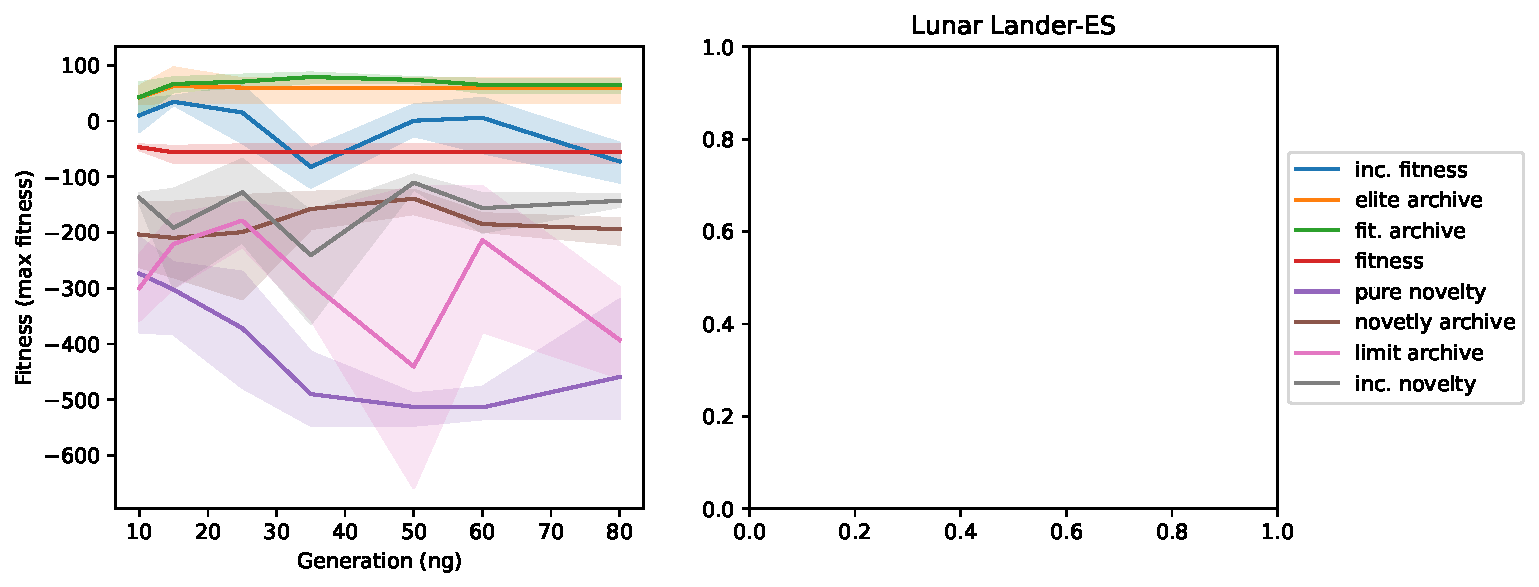
\includegraphics[width=0.8\textwidth]{../img/generations_lunarlander_lambda_max_fit.pdf}
	\caption{Maximal fitness performance characteristic of DE on LL.}
	\label{fig:fitness1}
\end{figure}
\begin{figure}[ht]
	\centering
	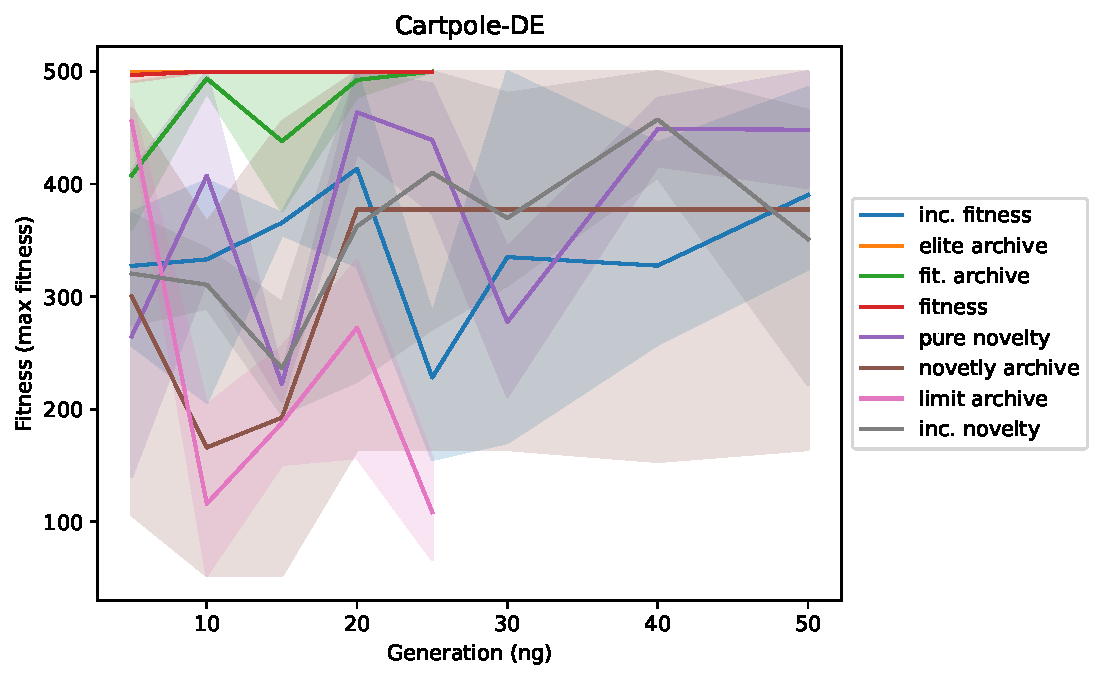
\includegraphics[width=0.8\textwidth]{../img/generations_cartpole_diff_max_fit.pdf}
	\caption{Maximal fitness performance characteristic of DE in Cartpole environment.}
	\label{fig:fitness2}
\end{figure}

\begin{figure}[ht]
	\centering
	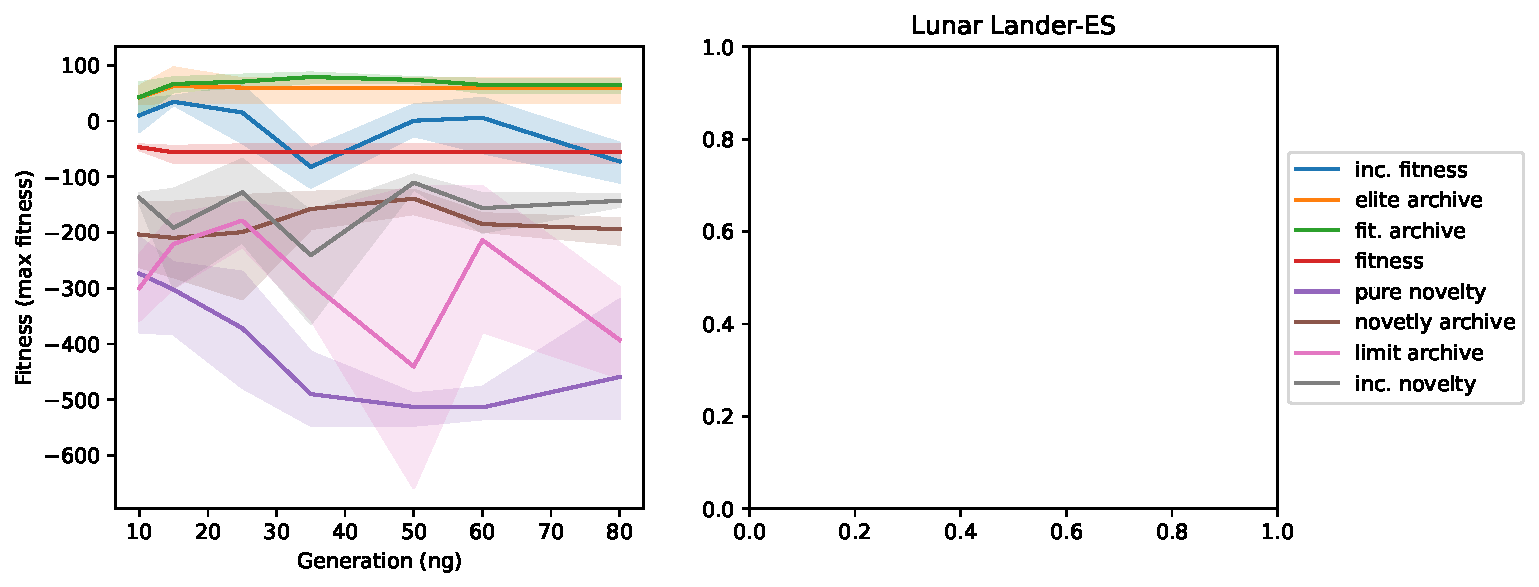
\includegraphics[width=0.8\textwidth]{../img/generations_lunarlander_lambda_max_fit.pdf}
	\caption{Maximal fitness performance characteristic of ES on LL.}
	\label{fig:fitness3}
\end{figure}
\begin{figure}[ht]
	\centering
	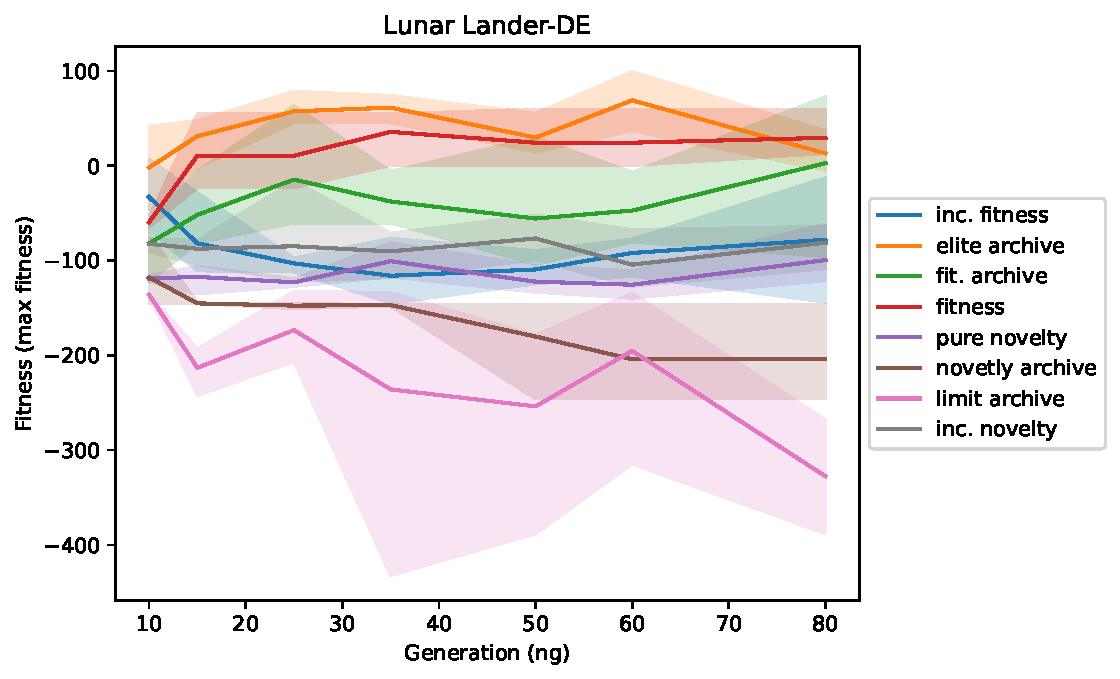
\includegraphics[width=0.8\textwidth]{../img/generations_lunarlander_diff_max_fit.pdf}
	\caption{Maximal fitness performance characteristic of DE on LL.}
	\label{fig:fitness4}
\end{figure}

\Crefrange{fig:fitness1}{fig:fitness4} however have been pruned for readability and do not represent the full range of values that have been taken into account such as the population median or mean. The shaded area represents quantiles $ q_{75} and q_{25} $ other values have been pruned. The actual scope of values considered for each contained is represented by chart that have been for readability sake put into \cref{app:generationGrid}. We evaluated the algorithm on 5 different seeds.

The hand-selected generation counts for the final evaluation are described in \cref{tab:gridResults}.  

\begin{table}[ht]
	\centering
	\scriptsize
	\setlength{\tabcolsep}{4pt}
	\renewcommand{\arraystretch}{1.15}
	\begin{tabular}{l||cc|cc}
		\toprule
		{} & \multicolumn{2}{l}{Lunar Lander} & \multicolumn{2}{l}{Cartpole} \\
		{} &           DE &  ES &       DE &  ES \\
		\midrule
		fitness         &           35 &  25 &       15 &  10 \\
		pure novelty    &           15 &  10 &       25 &  40 \\
		fit. archive    &           80 &  15 &       35 &  25 \\
		inc. fitness    &           15 &  15 &       15 &  20 \\
		inc. novelty    &           25 &  25 &       20 &  40 \\
		novetly archive &           25 &  60 &       20 &  20 \\
		elite archive   &           60 &  15 &       20 &  10 \\
		limit archive   &           25 &  25 &       20 &  20 \\
		\bottomrule
	\end{tabular}
	
	\caption{Selection of generations hyperparameter based on performed grid search}
	\label{tab:gridResults}
\end{table}

\section{Final Results}
After obtaining what we believe to be best performing available hyper-parameters for all containers, we apply this to the final round of tests. We will run the parameterised algorithms on 45 distinct seeds for each environment from which we collect data about the last population. We will subject the colect data to the statistical tests described in section \ref{sec:prefinalComp}. First we will test results of both evolutionary algorithms we have utilised (DE and ES) collected across all containers. Then we will test differences between the objective handling methods. Then we will group these methods based on objective used, following the internal divide in section \ref{sec:objFunc}. Since the groupings of results are different in each case, we claim them to be different test families for the purposes of ajdustments to  \textit{FWER}. 
    
\subsection{EA comparison}
Since we examine only two distinct EA implementations we have directly performed Wilcoxon test. First we see how the EAs performed on each of the environments separately. On both environments the Wilcoxon test rejects the null hypotesis with p values $ p_{LL} = 6.76 \times 10^{-11} $ and $ p_{CT} = 0.0002$ for Lunar lander and Cartpole respectively. On each of the enviroments we calculate the direction of the difference  through Hodges–Lehmann estimator over the differences $  d_i = ES_i - DE_i $. 
Directional values are $ HL_{LL} = -68.8 $ and $ HL_{CT} = 29.12 $ suggesting that DE has been more performant on Lunar lander while ES has been more performant on Cartpole.
Finally we pool the run from both environments and perform global Wilcox test. Unsuprisingly in the pooled cased we do not find enough evidence to reject $ H_0 $ ($ W_T = 60862$, $ p = 0.224$) as the per-environment performances largely cancel out. 
\subsection{Objective handling comparison}
Now we want to compare the objective handling methods based on fitness of individuals they have produced.
Friedman test rejects the null hypotesis for both Lunar Lander ($ \chi_F = 210.29 $, $ p_F = 7.57 \times 10^{-42} $) and Cartpole ($ \chi_F = 326.66 $, $ p_F = 1.21 \times 10^{-66} $). So we proceed to the pairwise Wilcoxon tests on both environments. The results are shown in \cref{tab:contWilcoxonLL,tab:contWilcoxonCT} respectively.

\begin{table}[ht]
	\centering
	\scriptsize
	\setlength{\tabcolsep}{4pt}
	\renewcommand{\arraystretch}{1.15}
	\resizebox{\textwidth}{!}{%
	\begin{tabular}{cc||ccccccc}
		\toprule
		A &               B &   $W_T$ &                     p &          HL &            $p_{Holm}$ &            $p_{Hoch}$ & Conclusion \\
		\midrule
		fitness &    pure novelty & 170.000 &  $4.15\times 10^{-8}$ &  128.843167 &  $6.22\times 10^{-7}$ &  $6.22\times 10^{-7}$ &   rejected \\
		fitness &    inc. fitness & 873.000 &                 0.928 &           - &                 1.000 &                 0.928 &  sustained \\
		fitness &    inc. novelty & 226.000 &  $3.93\times 10^{-7}$ &   92.643877 &  $4.72\times 10^{-6}$ &  $4.72\times 10^{-6}$ &   rejected \\
		fitness &    fit. archive & 765.000 &                 0.269 &           - &                 0.808 &                 0.808 &  sustained \\
		fitness &   elite archive & 686.000 &                 0.092 &           - &                 0.633 &                 0.434 &  sustained \\
		fitness & novetly archive &  71.000 & $5.19\times 10^{-10}$ &  139.303538 &  $1.04\times 10^{-8}$ &  $1.04\times 10^{-8}$ &   rejected \\
		fitness &   limit archive &  68.000 & $4.51\times 10^{-10}$ &  224.407512 &  $1.04\times 10^{-8}$ &  $1.04\times 10^{-8}$ &   rejected \\
		pure novelty &    inc. fitness & 149.000 &  $1.71\times 10^{-8}$ & -114.614712 &  $2.91\times 10^{-7}$ &  $2.91\times 10^{-7}$ &   rejected \\
		pure novelty &    inc. novelty & 685.000 &                 0.090 &           - &                 0.633 &                 0.434 &  sustained \\
		pure novelty &    fit. archive &  60.000 & $3.09\times 10^{-10}$ & -129.703835 &  $7.42\times 10^{-9}$ &  $7.42\times 10^{-9}$ &   rejected \\
		pure novelty &   elite archive &  70.000 & $4.95\times 10^{-10}$ & -147.305362 &  $1.04\times 10^{-8}$ &  $1.04\times 10^{-8}$ &   rejected \\
		pure novelty & novetly archive & 697.000 &                 0.109 &           - &                 0.633 &                 0.434 &  sustained \\
		pure novelty &   limit archive & 320.000 &  $1.19\times 10^{-5}$ &   91.802822 &  $1.30\times 10^{-4}$ &  $1.30\times 10^{-4}$ &   rejected \\
		inc. fitness &    inc. novelty & 190.000 &  $9.44\times 10^{-8}$ &   92.265044 &  $1.32\times 10^{-6}$ &  $1.32\times 10^{-6}$ &   rejected \\
		inc. fitness &    fit. archive & 686.000 &                 0.092 &           - &                 0.633 &                 0.434 &  sustained \\
		inc. fitness &   elite archive & 646.000 &                 0.048 &           - &                 0.381 &                 0.381 &  sustained \\
		inc. fitness & novetly archive &  69.000 & $4.73\times 10^{-10}$ &  145.000351 &  $1.04\times 10^{-8}$ &  $1.04\times 10^{-8}$ &   rejected \\
		inc. fitness &   limit archive &   9.000 & $2.56\times 10^{-11}$ &  227.153914 & $7.18\times 10^{-10}$ & $7.18\times 10^{-10}$ &   rejected \\
		inc. novelty &    fit. archive &  87.000 &  $1.09\times 10^{-9}$ & -108.043891 &  $1.96\times 10^{-8}$ &  $1.96\times 10^{-8}$ &   rejected \\
		inc. novelty &   elite archive & 165.000 &  $3.37\times 10^{-8}$ & -128.079075 &  $5.39\times 10^{-7}$ &  $5.39\times 10^{-7}$ &   rejected \\
		inc. novelty & novetly archive & 437.000 &  $4.33\times 10^{-4}$ &   39.747988 &                 0.004 &                 0.004 &   rejected \\
		inc. novelty &   limit archive & 196.000 &  $1.20\times 10^{-7}$ &  120.348414 &  $1.56\times 10^{-6}$ &  $1.56\times 10^{-6}$ &   rejected \\
		fit. archive &   elite archive & 837.000 &                 0.566 &           - &                 1.000 &                 0.928 &  sustained \\
		fit. archive & novetly archive &  54.000 & $2.32\times 10^{-10}$ &  159.409308 &  $5.81\times 10^{-9}$ &  $5.81\times 10^{-9}$ &   rejected \\
		fit. archive &   limit archive &  15.000 & $3.46\times 10^{-11}$ &  244.356882 & $9.35\times 10^{-10}$ & $9.35\times 10^{-10}$ &   rejected \\
		elite archive & novetly archive &  74.000 & $5.97\times 10^{-10}$ &   168.11856 &  $1.14\times 10^{-8}$ &  $1.14\times 10^{-8}$ &   rejected \\
		elite archive &   limit archive &  28.000 & $6.59\times 10^{-11}$ &  248.159355 &  $1.71\times 10^{-9}$ &  $1.71\times 10^{-9}$ &   rejected \\
		novetly archive &   limit archive & 396.000 &  $1.33\times 10^{-4}$ &   77.327852 &                 0.001 &                 0.001 &   rejected \\
		\bottomrule
	\end{tabular}
	}	
	\caption{Fitness Wilcoxon test over objectives handlers for Lunar Lander}
	\label{tab:contWilcoxonLL}
\end{table}

\begin{table}[ht]
	\centering
	\scriptsize
	\setlength{\tabcolsep}{4pt}
	\renewcommand{\arraystretch}{1.15}
	\resizebox{\textwidth}{!}{%
\begin{tabular}{cc||ccccccc}
	\toprule
	A &               B &    $W_T$ &                     p &          HL &            $p_{Holm}$ &            $p_{Hoch}$ & Conclusion \\
	\midrule
	fitness &    pure novelty &   50.000 & $3.85\times 10^{-13}$ &  179.666667 & $6.54\times 10^{-12}$ & $6.54\times 10^{-12}$ &   rejected \\
	fitness &    inc. fitness &  198.500 &  $2.20\times 10^{-7}$ &   79.916667 &  $2.86\times 10^{-6}$ &  $2.86\times 10^{-6}$ &   rejected \\
	fitness &    inc. novelty &   66.000 & $4.01\times 10^{-14}$ &  195.416667 & $8.41\times 10^{-13}$ & $8.41\times 10^{-13}$ &   rejected \\
	fitness &    fit. archive &  324.000 &                 0.111 &           - &                 0.444 &                 0.444 &  sustained \\
	fitness &   elite archive &  138.500 &                 0.088 &           - &                 0.438 &                 0.438 &  sustained \\
	fitness & novetly archive &   11.000 & $1.73\times 10^{-15}$ &       287.5 & $4.66\times 10^{-14}$ & $4.66\times 10^{-14}$ &   rejected \\
	fitness &   limit archive &   70.000 & $2.03\times 10^{-14}$ &  212.666667 & $4.47\times 10^{-13}$ & $4.47\times 10^{-13}$ &   rejected \\
	pure novelty &    inc. fitness &  987.000 &  $2.31\times 10^{-4}$ &      -97.25 &                 0.002 &                 0.002 &   rejected \\
	pure novelty &    inc. novelty & 1553.000 &                 0.229 &           - &                 0.687 &                 0.604 &  sustained \\
	pure novelty &    fit. archive &  118.000 & $2.15\times 10^{-12}$ & -168.083333 & $3.43\times 10^{-11}$ & $3.43\times 10^{-11}$ &   rejected \\
	pure novelty &   elite archive &   34.000 & $1.38\times 10^{-13}$ & -190.083333 & $2.48\times 10^{-12}$ & $2.48\times 10^{-12}$ &   rejected \\
	pure novelty & novetly archive & 1149.500 &  $3.02\times 10^{-4}$ &  108.416667 &                 0.003 &                 0.002 &   rejected \\
	pure novelty &   limit archive & 1710.000 &                 0.302 &           - &                 0.687 &                 0.604 &  sustained \\
	inc. fitness &    inc. novelty &  733.500 &  $2.74\times 10^{-6}$ &       110.5 &  $3.29\times 10^{-5}$ &  $3.29\times 10^{-5}$ &   rejected \\
	inc. fitness &    fit. archive &  444.000 &  $8.41\times 10^{-6}$ &  -63.416667 &  $9.25\times 10^{-5}$ &  $9.25\times 10^{-5}$ &   rejected \\
	inc. fitness &   elite archive &   27.000 & $3.19\times 10^{-10}$ &  -86.083333 &  $4.79\times 10^{-9}$ &  $4.79\times 10^{-9}$ &   rejected \\
	inc. fitness & novetly archive &  149.000 & $8.01\times 10^{-14}$ &  200.333333 & $1.52\times 10^{-12}$ & $1.52\times 10^{-12}$ &   rejected \\
	inc. fitness &   limit archive &  520.000 &  $2.19\times 10^{-9}$ &  128.083333 &  $3.06\times 10^{-8}$ &  $3.06\times 10^{-8}$ &   rejected \\
	inc. novelty &    fit. archive &   44.000 & $6.07\times 10^{-14}$ &      -182.5 & $1.21\times 10^{-12}$ & $1.21\times 10^{-12}$ &   rejected \\
	inc. novelty &   elite archive &   16.000 & $1.43\times 10^{-14}$ & -204.333333 & $3.44\times 10^{-13}$ & $3.44\times 10^{-13}$ &   rejected \\
	inc. novelty & novetly archive & 1115.000 &  $2.82\times 10^{-4}$ &   87.416667 &                 0.003 &                 0.002 &   rejected \\
	inc. novelty &   limit archive & 1930.000 &                 0.636 &           - &                 0.687 &                 0.636 &  sustained \\
	fit. archive &   elite archive &  134.000 &                 0.001 &         0.0 &                 0.006 &                 0.006 &   rejected \\
	fit. archive & novetly archive &   18.000 & $2.21\times 10^{-15}$ &  276.083333 & $5.75\times 10^{-14}$ & $5.75\times 10^{-14}$ &   rejected \\
	fit. archive &   limit archive &   86.000 & $1.54\times 10^{-14}$ &       198.5 & $3.54\times 10^{-13}$ & $3.54\times 10^{-13}$ &   rejected \\
	elite archive & novetly archive &    5.000 & $1.39\times 10^{-15}$ &  302.833333 & $3.90\times 10^{-14}$ & $3.90\times 10^{-14}$ &   rejected \\
	elite archive &   limit archive &   27.000 & $3.04\times 10^{-15}$ &  220.833333 & $7.59\times 10^{-14}$ & $7.59\times 10^{-14}$ &   rejected \\
	novetly archive &   limit archive & 1164.000 &  $3.78\times 10^{-4}$ &  -68.416667 &                 0.003 &                 0.003 &   rejected \\
	\bottomrule
\end{tabular}
}
	\caption{Fitness Wilcoxon test over objectives handlers for Cartpole}
	\label{tab:contWilcoxonCT}
\end{table}
\subsection{Diversity Comparison}
Now that we have made the comparison on achieved fitness we want to compare the algorithms also based on the produced diversity.
The Friedman test rejects the null hypotesis also for divirsities both for Lunar Lander ($ \chi_F = 192.23 $, $ p_F = 5 \times 10^{-38} $) and Cartpole ($ \chi_F = 163.918 $, $ p_F = 4.8 \times 10^{-32} $) and so we can safely perform Wilcoxon test on the combinations of objective handling methods. Results are shown in \cref{tab:contWilcoxonCTDiv,tab:contWilcoxonLLDiv}.

\begin{table}[ht]
	\centering
	\scriptsize
	\setlength{\tabcolsep}{4pt}
	\renewcommand{\arraystretch}{1.15}
	\resizebox{\textwidth}{!}{%
		\begin{tabular}{lcccccccc}
			\toprule
			A &               B &   $W_T$ &                     p &        HL &            $p_{Holm}$ &            $p_{Hoch}$ & Conclusion \\
			\midrule
			fitness &    pure novelty & 1323.00 &                  0.00 & -0.042555 &                  0.04 &                  0.04 &   rejected \\
			fitness &    inc. fitness &  947.00 &  $9.51\times 10^{-6}$ &  0.090809 &  $1.33\times 10^{-4}$ &  $1.33\times 10^{-4}$ &   rejected \\
			fitness &    inc. novelty & 1640.00 &                  0.10 &         - &                  0.51 &                  0.51 &  sustained \\
			fitness &    fit. archive & 1183.00 &  $5.04\times 10^{-4}$ &  0.073376 &                  0.01 &                  0.01 &   rejected \\
			fitness &   elite archive &  189.00 & $7.54\times 10^{-14}$ &  0.217708 & $2.04\times 10^{-12}$ & $2.04\times 10^{-12}$ &   rejected \\
			fitness & novetly archive &  650.00 &  $1.88\times 10^{-8}$ &  0.225698 &  $3.94\times 10^{-7}$ &  $3.94\times 10^{-7}$ &   rejected \\
			fitness &   limit archive &  829.00 &  $9.44\times 10^{-7}$ &  0.146048 &  $1.70\times 10^{-5}$ &  $1.70\times 10^{-5}$ &   rejected \\
			pure novelty &    inc. fitness &  735.00 &  $1.28\times 10^{-7}$ &  0.149859 &  $2.57\times 10^{-6}$ &  $2.57\times 10^{-6}$ &   rejected \\
			pure novelty &    inc. novelty & 1941.00 &                  0.67 &         - &                  1.00 &                  0.84 &  sustained \\
			pure novelty &    fit. archive &  464.00 & $1.87\times 10^{-10}$ &  0.129778 &  $4.31\times 10^{-9}$ &  $4.31\times 10^{-9}$ &   rejected \\
			pure novelty &   elite archive &   45.00 & $7.79\times 10^{-16}$ &  0.262882 & $2.18\times 10^{-14}$ & $2.18\times 10^{-14}$ &   rejected \\
			pure novelty & novetly archive &  271.00 & $8.80\times 10^{-13}$ &  0.272268 & $2.29\times 10^{-11}$ & $2.29\times 10^{-11}$ &   rejected \\
			pure novelty &   limit archive &  393.00 & $2.79\times 10^{-11}$ &   0.19342 & $6.70\times 10^{-10}$ & $6.70\times 10^{-10}$ &   rejected \\
			inc. fitness &    inc. novelty &  930.00 &  $6.91\times 10^{-6}$ & -0.114747 &  $1.04\times 10^{-4}$ &  $1.04\times 10^{-4}$ &   rejected \\
			inc. fitness &    fit. archive & 1804.00 &                  0.33 &         - &                  0.98 &                  0.84 &  sustained \\
			inc. fitness &   elite archive &  959.00 &  $1.19\times 10^{-5}$ &  0.122055 &  $1.54\times 10^{-4}$ &  $1.54\times 10^{-4}$ &   rejected \\
			inc. fitness & novetly archive & 1354.00 &                  0.01 &  0.125952 &                  0.05 &                  0.05 &   rejected \\
			inc. fitness &   limit archive & 1754.00 &                  0.24 &         - &                  0.95 &                  0.84 &  sustained \\
			inc. novelty &    fit. archive &  923.00 &  $6.05\times 10^{-6}$ &  0.111492 &  $9.68\times 10^{-5}$ &  $9.68\times 10^{-5}$ &   rejected \\
			inc. novelty &   elite archive &  283.00 & $1.25\times 10^{-12}$ &  0.243282 & $3.12\times 10^{-11}$ & $3.12\times 10^{-11}$ &   rejected \\
			inc. novelty & novetly archive &  596.00 &  $5.21\times 10^{-9}$ &  0.240971 &  $1.15\times 10^{-7}$ &  $1.15\times 10^{-7}$ &   rejected \\
			inc. novelty &   limit archive &  863.00 &  $1.88\times 10^{-6}$ &  0.171545 &  $3.19\times 10^{-5}$ &  $3.19\times 10^{-5}$ &   rejected \\
			fit. archive &   elite archive &  825.00 &  $8.70\times 10^{-7}$ &  0.137525 &  $1.65\times 10^{-5}$ &  $1.65\times 10^{-5}$ &   rejected \\
			fit. archive & novetly archive &  975.00 &  $1.59\times 10^{-5}$ &  0.141326 &  $1.91\times 10^{-4}$ &  $1.91\times 10^{-4}$ &   rejected \\
			fit. archive &   limit archive & 1502.00 &                  0.03 &         - &                  0.17 &                  0.17 &  sustained \\
			elite archive & novetly archive & 1952.00 &                  0.84 &         - &                  1.00 &                  0.84 &  sustained \\
			elite archive &   limit archive & 1482.00 &                  0.02 &         - &                  0.16 &                  0.16 &  sustained \\
			novetly archive &   limit archive & 1309.00 &                  0.02 &         - &                  0.12 &                  0.12 &  sustained \\
			\bottomrule
		\end{tabular}
	}
	\caption{Diversity Wilcoxon test over objectives handlers for Cartpole}
	\label{tab:contWilcoxonCTDiv}
\end{table}

\begin{table}[ht]
	\centering
	\scriptsize
	\setlength{\tabcolsep}{4pt}
	\renewcommand{\arraystretch}{1.15}
	\resizebox{\textwidth}{!}{%
		\begin{tabular}{lcccccccc}
			\toprule
			A &               B &  $W_T$ &                     p &        HL &            $p_{Holm}$ &            $p_{Hoch}$ & Conclusion \\
			\midrule
			fitness &    pure novelty &  49.00 & $1.83\times 10^{-10}$ & -0.102046 &  $4.20\times 10^{-9}$ &  $4.20\times 10^{-9}$ &   rejected \\
			fitness &    inc. fitness & 119.00 &  $1.18\times 10^{-8}$ & -0.069382 &  $2.60\times 10^{-7}$ &  $2.60\times 10^{-7}$ &   rejected \\
			fitness &    inc. novelty & 122.00 &  $2.18\times 10^{-8}$ & -0.075654 &  $4.57\times 10^{-7}$ &  $4.57\times 10^{-7}$ &   rejected \\
			fitness &    fit. archive & 501.00 &                  0.04 &         - &                  0.26 &                  0.26 &  sustained \\
			fitness &   elite archive &  59.00 &  $1.44\times 10^{-7}$ &  0.066169 &  $2.44\times 10^{-6}$ &  $2.44\times 10^{-6}$ &   rejected \\
			fitness & novetly archive & 273.00 &  $2.29\times 10^{-6}$ & -0.119972 &  $3.43\times 10^{-5}$ &  $3.43\times 10^{-5}$ &   rejected \\
			fitness &   limit archive & 609.00 &                  0.25 &         - &                  1.00 &                  0.71 &  sustained \\
			pure novelty &    inc. fitness & 600.00 &                  0.02 &         - &                  0.18 &                  0.18 &  sustained \\
			pure novelty &    inc. novelty & 709.00 &                  0.13 &         - &                  0.65 &                  0.65 &  sustained \\
			pure novelty &    fit. archive & 383.00 &  $8.99\times 10^{-5}$ &  0.082667 &                  0.00 &                  0.00 &   rejected \\
			pure novelty &   elite archive &      0 & $1.63\times 10^{-11}$ &  0.179489 & $4.56\times 10^{-10}$ & $4.56\times 10^{-10}$ &   rejected \\
			pure novelty & novetly archive & 865.00 &                  0.71 &         - &                  1.00 &                  0.71 &  sustained \\
			pure novelty &   limit archive &  25.00 & $5.68\times 10^{-11}$ &  0.123138 &  $1.53\times 10^{-9}$ &  $1.53\times 10^{-9}$ &   rejected \\
			inc. fitness &    inc. novelty & 778.00 &                  0.42 &         - &                  1.00 &                  0.71 &  sustained \\
			inc. fitness &    fit. archive & 586.00 &                  0.02 &         - &                  0.19 &                  0.19 &  sustained \\
			inc. fitness &   elite archive &  11.00 & $6.22\times 10^{-11}$ &  0.141697 &  $1.55\times 10^{-9}$ &  $1.55\times 10^{-9}$ &   rejected \\
			inc. fitness & novetly archive & 694.00 &                  0.10 &         - &                  0.62 &                  0.62 &  sustained \\
			inc. fitness &   limit archive & 169.00 &  $1.07\times 10^{-7}$ &  0.087411 &  $2.03\times 10^{-6}$ &  $2.03\times 10^{-6}$ &   rejected \\
			inc. novelty &    fit. archive & 505.00 &                  0.00 &  0.059472 &                  0.05 &                  0.05 &   rejected \\
			inc. novelty &   elite archive &   1.00 & $7.97\times 10^{-11}$ &  0.148144 &  $1.91\times 10^{-9}$ &  $1.91\times 10^{-9}$ &   rejected \\
			inc. novelty & novetly archive & 809.00 &                  0.44 &         - &                  1.00 &                  0.71 &  sustained \\
			inc. novelty &   limit archive & 197.00 &  $3.43\times 10^{-7}$ &  0.099544 &  $5.48\times 10^{-6}$ &  $5.48\times 10^{-6}$ &   rejected \\
			fit. archive &   elite archive & 125.00 &  $2.50\times 10^{-8}$ &  0.102542 &  $4.99\times 10^{-7}$ &  $4.99\times 10^{-7}$ &   rejected \\
			fit. archive & novetly archive & 358.00 &  $4.12\times 10^{-5}$ & -0.078927 &  $5.36\times 10^{-4}$ &  $5.36\times 10^{-4}$ &   rejected \\
			fit. archive &   limit archive & 491.00 &                  0.00 &  0.052381 &                  0.05 &                  0.05 &   rejected \\
			elite archive & novetly archive &  26.00 & $5.97\times 10^{-11}$ & -0.188639 &  $1.55\times 10^{-9}$ &  $1.55\times 10^{-9}$ &   rejected \\
			elite archive &   limit archive & 181.00 &  $1.77\times 10^{-5}$ & -0.048803 &  $2.48\times 10^{-4}$ &  $2.48\times 10^{-4}$ &   rejected \\
			novetly archive &   limit archive & 198.00 &  $1.30\times 10^{-7}$ &  0.134406 &  $2.35\times 10^{-6}$ &  $2.35\times 10^{-6}$ &   rejected \\
			\bottomrule
		\end{tabular}
	}
	\caption{Diversity Wilcoxon test over objectives handlers for Lunar Lander}
	\label{tab:contWilcoxonLLDiv}
\end{table}
\subsection{Group comparison}
We woul also like to compare the groups based on objective as such (fitness, novelty, combination). For that we wan to assess the group cohesion in each of th 
\section{Discussion}
